\creaCapitulo{OpenMP}

OpenMP es un modelo de programación paralela para arquitecturas de memoria compartida, diseñado para proporcionar una interfaz portable, escalable y de alto nivel que permita explotar el paralelismo en CPUs multinúcleo sin recurrir a APIs de hilos de bajo nivel. Su diseño se basa en directivas de compilador, rutinas de biblioteca y variables de entorno, y sigue el modelo de ejecución \textit{fork–join}, donde un hilo maestro crea y sincroniza equipos de hilos que ejecutan regiones paralelas. \cite{Jin2024}

Surge en 1997, cuando Intel impulsa la creación del OpenMP Architecture Review Board (ARB), un consorcio formado por fabricantes de hardware y software (Intel, IBM, AMD, HP, Nvidia, Oracle, entre otros) con el objetivo de definir un estándar común para paralelismo en memoria compartida. La última versión de OpenMP, la 6.0, data de 2024.

OpenMP implementa paralelismo mediante \textit{multithreading}. El funcionamiento es relativamente simple, el programa comienza con un comportamiento secuencial y un hilo maestro. Cuando este hilo se encuentra una región paralela con \textit{\#pragma omp parallel}, se crea un equipo de hilos \cite{ARB2024}. Los hilos ejecutan el bloque paralelo de forma concurrente, y al finalizar, los hilos se unen y el control vuelve al maestro.

Podemos identificar se compone de varios elementos principales, el primero de los cuales sería las directivas de compilador, como \textit{\#pragma omp parallel}, \textit{\#pragma omp for}, o \textit{\#pragma omp single}, y sus cláusulas como \textit{schedule}, \textit{shared}, o \textit{default}. Otros elementos importantes son las funciones de biblioteca, como \textit{omp\_set\_num\_threads()} o \textit{omp\_get\_wtime()}, y las variables de entorno, como \textit{OMP\_NUM\_THREADS}, \textit{OMP\_SCHEDULE}, o \textit{OMP\_DYNAMIC}. \cite{ARB2024} 

Como hemos comentado, OpenMP opera sobre un modelo de memoria compartida en la que todos los hilos ven el mismo espacio de direcciones, en el que las variables pueden ser visibles por todos los hilos ($shared$), o cada hilo tiene su propia copia ($private$). Este modelo evita la necesidad de comunicación explícita entre procesos (como en MPI), simplificando el desarrollo. \cite{Jin2024}

\creaSeccion{Implementación Secuencial}

Tomaremos como punto de partida la implementación secuencial de los problemas \cite{Mantas2024}, de la cual ya disponemos.

\begin{figure}[H]
	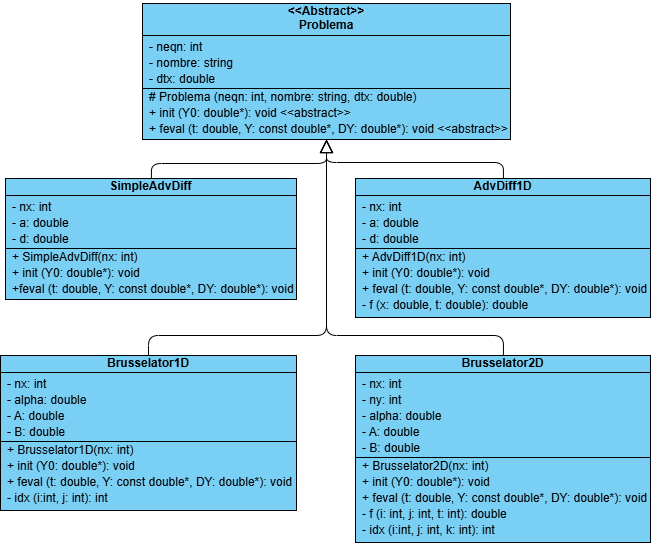
\includegraphics[width=\linewidth]{imagenes/OMP-Diagrama-Problemas.png}
	\caption{Diagrama de Clases de los problemas OMP}
	\label{fig:OMP-Diagrama-Problemas}
\end{figure}

Como comentamos anteriormente, no nos centraremos en la resolución de los problemas \textit{per se}, puesto que ésta se nos da ya hecha y corregida, sino que nuestros esfuerzos irán en implementar los métodos de resolución en ambas formas de paralelismo, y buscar la máxima eficiencia. Para facilitar la implementación y la cohesión del código, definimos una clase abstracta \textit{Problema} de la cual heredarán los cuatro problemas.

El siguiente paso, por tanto, será realizar una implementación secuencial de los métodos, partiendo de los algoritmos que previamente hemos comentado, Runge-Kutta, Adams-Bashford, y Adamd-Bashford-Moulton, a saber, algoritmos \ref{alg:RungeKutta4}, \ref{alg:AdamsBashford}, y \ref{alg:AdamsBashfordMoulton}, respectivamente. El lenguaje elegido será C++, para luego poder añadir la parte de OpenMP o CUDA.

\begin{figure}[H]
	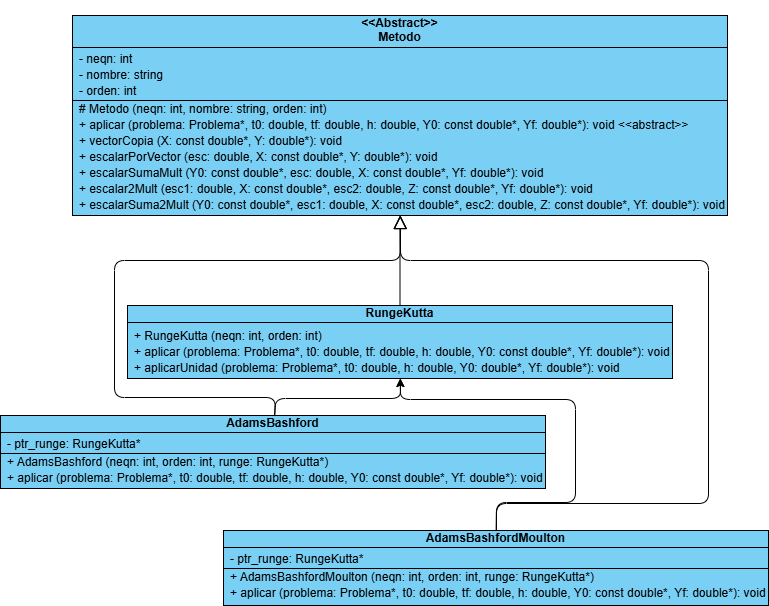
\includegraphics[width=\linewidth]{imagenes/OMP-Diagrama-Metodos.png}
	\caption{Diagrama de Clases de los métodos OMP}
	\label{fig:OMP-Diagrama-Metodos}
\end{figure}

El planteamiento que se hace con los métodos es similar al de los problemas, una clase abstracta padre de la cual puedan heredar los métodos. Además, en la clase padre \textit{Metodo} hemos implementado diversas funciones auxiliares que nos van a facilitar el trabajar con vectores. Con este diseño, a través de la herencia y el polimorfismo, podríamos aumentar el alcance de nuestro proyecto añadiendo nuevos métodos o más problemas sin dificultad ninguna.

Ahora que tenemos una primera maqueta funcional (aunque poco eficiente), podremos comenzar con el trabajo en paralelo. De cara a nuestro proyecto, lo primero que debemos tener en cuenta es que no podemos simplemente paralelizar el bucle principal con el que trabajamos (e.g. el bucle while en el algoritmo \ref{alg:AdamsBashford}) porque cada iteración necesita de la anterior para calcular el siguiente paso. Deberemos buscar por tanto otras formas de atacar el problema. En el caso de OpenMP hemos planteado dos formas, paralelismo por operaciones, y por componentes.

\creaSeccion{Paralelismo por Operaciones}

En esta estrategia buscamos que cada función paralelice su propio trabajo. Eso quiere decir que cada operación vectorial, como el \textit{feval()}, o \textit{escalarPorVector}, tiene su propio \textit{\#pragma omp parallel}, crea un equipo de hilos, reparte el trabajo, y lo sincroniza.

De forma simplificada, veamos un ejemplo de Adams-Bashford 4:

\begin{algorithm}[H]
	\begin{algorithmic}
		\State $ Y_{n0} \gets Y_0 $
		\State $ Y_n \gets arranqueRK4(Y_{n-1})$ \Comment{$ n = \{1, 2, 3\} $}
		\State $ F_n \gets feval(t_n\text{, }Y_n)$ \Comment{$ n = \{0, 1, 2, 3\} $}
		\For{ $ t_n \text{=} t_0 \text{+} 3h \text{; }t_n < t_f\text{; }t_n \text{+=}h $ }
			\State $ escalar2Mult(37.0\text{, }F_{n1}\text{, -}9.0\text{, }F_{n0}\text{, }Y_{aux}) $
			\State $ escalarSuma2Mult( Y_{aux}\text{, }55.0\text{, }F_{n3}\text{, -}59.0\text{, }F_{n2}\text{, }Y_{aux} ) $
			\State $ escalarSumaMult( Y_{n3}\text{, }h/24.0\text{, }Y_{aux}\text{, }Y_{n4} ) $
			\State $ F_{n4} \gets feval(t_n+h\text{, }Y_{n4}) $
			
			\State $ swap(Y_{n4}\text{, }Y_{n3}) $
			\State $ swap(F_n\text{, }F_{n-1}) $ \Comment{$ n = \{1, 2, 3, 4\} $}
		\EndFor
		\State $Y_f \gets Y_{n3}$
	\end{algorithmic}
	\caption{Implementación de AB4 con Paralelismo por Operaciones}
	\label{alg:AB4ParalelismoOperaciones}
\end{algorithm}

Como podemos ver, para hacer el cálculo propio de Adams-Bashford de orden 4 (ecuación \ref{eq:AdamsBashford4}) la hemos divido en 3 partes utilizando las funciones auxiliares de la clase abstracta \textit{Metodo} de las que ya disponíamos. Dentro de cada una de ellas se creará el grupo de hilos, se repartirá el trabajo (cada hilo tendrá un "trozo" de vector sobre el que trabajar), y una vez finalicen se sincronizará para retornar a la función principal. Por ejemplo, \textit{vectorCopia()}:
\begin{algorithm}[H]
	\begin{algorithmic}
		\State \verb|#pragma omp parallel for schedule(static)|
		\For{ $ i \text{=} 0 \text{; }i < neqn\text{; }\text{++}i $ }
			\State $ Y[i] \gets X[i] $
		\EndFor
		
	\end{algorithmic}
	\caption{Implementación de Función Auxiliar vectorCopia}
	\label{alg:VectorCopia-OMP}
\end{algorithm}

Esta estrategia trae consigo ventajas como la modularidad, ya que cada operación vectorial es independiente y autocontenida, lo cual facilita la depuración y la legibilidad del código.

El principal punto negativo de esta estrategia es que trae consigo un \textit{overhead} alto, ya que cada función tiene una barrera implícita al acabar un \textit{parallel for}, en cada iteración del bucle hay varias llamadas a funciones, y el bucle itera un elevado número de veces. Esto equivale a más paradas de las que serían deseadas, además de que los hilos entran y salen de regiones paralelas constantemente.

\creaSeccion{Paralelismo por Componentes}

Frente al paralelismo de operaciones, tenemos el paralelismo por componentes (o por elementos), en el que sólo tenemos una gran región \textit{parallel} dentro de la cual ocurre todo el paralelismo, y cada hebra calcula su parte de los vectores.

Esto quiere decir que se creará un único equipo de hilos al entrar en el \textit{parallel}, y todos los hilos permanecerán activos e iterarán en el bucle, paso a paso. Dentro del bucle iterativo, habrá diversos \textit{\#pragma omp for} que repartirán los índices entre los hilos. Esto además nos permitirá reducir las barreras de sincronización. Para poder comparar con la anterior implementación \ref{alg:AB4ParalelismoOperaciones}, describimos el mismo algoritmo (\ref{eq:AdamsBashford4}) pero con esta estrategia:

\begin{algorithm}[H]
	\begin{algorithmic}
		\State $ Y_{n0} \gets Y_0 $
		\State $ Y_n \gets arranqueRK4(Y_{n-1})$ \Comment{$ n = \{1, 2, 3\} $}
		\State \verb|#pragma omp parallel for schedule(static)|
		\For{ $ i \text{=} 0 \text{; }i < neqn\text{; }\text{++}i $ }
			\State $ F_n[i] \gets feval\_i(t_n\text{, }Y_n\text{, }i)$ \Comment{$ n = \{0, 1, 2, 3\} $}
		\EndFor
		
		\State \verb|#pragma omp parallel|
		\For{ $ t_n \text{=} t_0 \text{+} 3h \text{; }t_n < t_f\text{; }t_n \text{+=}h $ }
			\State \verb|#pragma omp for schedule(static)|
			\For{ $ i \text{=} 0 \text{; }i < neqn\text{; }\text{++}i $ }
				\State $ Y_4[i] = Y_3[i] + h/24 * ( 55F_3[i] - 59F_2[i] + 37F_1[i] -9F_0[i]) $
			\EndFor
			\State \verb|#pragma omp for schedule(static)|
			\For{ $ i \text{=} 0 \text{; }i < neqn\text{; }\text{++}i $ }
				\State $ F_4[i] \gets feval\_i(t_n+h\text{, }Y_4\text{, }i)$
			\EndFor
			\State \verb|#pragma omp single|
			\State $ swap(Y_{n4}\text{, }Y_{n3}) $
			\State $ swap(F_n\text{, }F_{n-1}) $ \Comment{$ n = \{1, 2, 3, 4\} $}
		\EndFor
		\State $Y_f \gets Y_{n3}$
	\end{algorithmic}
	\caption{Implementación de AB4 con Paralelismo por Componentes}
	\label{alg:AB4ParalelismoComponentes}
\end{algorithm}

La idea principal detrás de esta estrategia es reducir el \textit{overhead} provocado por tener demasiadas barreras de sincronización, y mejorar el uso de la caché. Para mejorar la implementación hacemos uso de directivas como \textit{schedule (static)}, con la que indicamos cómo deben repartirse las iteraciones entre los hilos. En este caso, se divide el rango de iteraciones en bloques contiguos y de tamaño fijo, y se asigna cada bloque a un hilo antes de empezar la ejecución del bucle. Esto es práctico cuando sabemos de antemano que todas las iteraciones van a costar lo mismo, y no va haber ramas pesadas o irregulares.

Algunas de las desventajas que tendremos es que el código es más complejo, pues no se puede reutilizar el \textit{feval()} secuencial (que sí lo aprovechábamos en el paralelismo por operaciones), sino que hay que hacer una versión específica para los componentes. De igual manera, no se pueden utilizar las funciones auxiliares, porque están diseñadas para tratar los vectores completos, no elementos individuales.

\creaSeccion{Mediciones}

Ante la pregunta de qué estrategia es mejor, la respuesta sería, como casi siempre en informática, que depende.

En un primer planteamiento, parece que el paralelismo por componentes debería ser mejor. Reduce la creación y destrucción repetitiva de las hebras, y reduce las barreras de sincronización.

Un matiz importante que debemos hacer es que, aunque hablemos de creación y destrucción de hilos iterativa, no siempre ha de ocurrir así. Es cierto que, de forma lógica, el modelo \textit{fork-join} de OpenMP describe de esa forma el comportamiento de los hilos; se crean, se usan, se destruyen. \cite{Jin2024} Sin embargo, esto no siempre ocurre así (ya que sería muy costoso).

Existe un concepto llamado \textit{thread pooling}, que describe que el entorno de ejecución podrá devolver los hilos a la \textit{pool} en lugar de destruirlos, y así ahorrarse crearlos posteriormente. \cite{Barlas2023} Esto eliminaría la principal desventaja del paralelismo por operaciones. 

De forma análoga, el \textit{runtime} no siempre mantiene los hilos activos (como pudiera parecer), aunque no haya finalizado el bloque \textit{parallel}, ya que si el trabajo dentro de cada bloque \textit{omp for} es pequeño, el compilador puede decidir dormir los hilos para ahorrar energía. Esto puede provocar pérdida de tiempo al tener que despertar los hilos, y latencias de sincronización más altas.

Otro dato a tener en cuenta, es que en el planteamiento de nuestros problemas, las llamadas a \textit{feval\_i()} son muy baratas, y el trabajo por iteración es pequeño, mientras que \textit{feval()} es más pesado, y en cierta forma se amortiza el \textit{overhead} al hacerse  una única llamada en lugar de \textit{neqn} llamadas.

Podemos comenzar, por ejemplo, comparando los tiempos al resolver el problema \textit{Brusselator1D} con 100.000 ecuaciones.
\begin{table}[H]
	\begin{center}
		\begin{tabular}{| c | c | c | c |}
			\hline
			\textbf{Solver} & \textbf{Hebras} & \textbf{Estrategia} & \textbf{T (s)} \\
			\hline
			
			% ---------------- RUNGE KUTTA ----------------
			\multirow{6}{*}{Runge-Kutta}
			& \multirow{2}{*}{1}  & OMP Componentes   & 2501.84 \\
			\cline{3-4}
			&                     & OMP Operaciones & 1544.87 \\
			\cline{2-4}
			& \multirow{2}{*}{4}  & OMP Componentes   & 670.504 \\
			\cline{3-4}
			&                     & OMP Operaciones & 371.93 \\
			\cline{2-4}
			& \multirow{2}{*}{16} & OMP Componentes   & 197.065 \\
			\cline{3-4}
			&                     & OMP Operaciones & 180.327 \\
			\hline
			
			% ---------------- ADAMS BASHFORD ----------------
			\multirow{6}{*}{Adams-Bashford}
			& \multirow{2}{*}{1}  & OMP Componentes   & 707.634 \\
			\cline{3-4}
			&                     & OMP Operaciones & 556.051 \\
			\cline{2-4}
			& \multirow{2}{*}{4}  & OMP Componentes   & 179.559 \\
			\cline{3-4}
			&                     & OMP Operaciones & 130.993 \\
			\cline{2-4}
			& \multirow{2}{*}{16} & OMP Componentes   & 56.5174 \\
			\cline{3-4}
			&                     & OMP Operaciones & 66.1485 \\
			\cline{3-4}
			\hline
			
			% ---------------- ADAMS BASHFORD MOULTON ----------------
			\multirow{6}{*}{Adams-Bashford-Moulton}
			& \multirow{2}{*}{1}  & OMP Componentes   & 2914.04 \\
			\cline{3-4}
			&                     & OMP Operaciones & 1772.73 \\
			
			\cline{2-4}
			& \multirow{2}{*}{4}  & OMP Componentes   & 785.555 \\
			\cline{3-4}
			&                     & OMP Operaciones & 438.018 \\
			
			\cline{2-4}
			& \multirow{2}{*}{16} & OMP Componentes   & 237.236 \\
			\cline{3-4}
			&                     & OMP Operaciones & 219.918 \\
			
			\hline
			
		\end{tabular}
		\caption{Tiempos de Brusselator1D con 100000 ecuaciones}
		\label{tab:Brusselator1D-100K}
	\end{center}
\end{table}

\begin{figure}[H]
	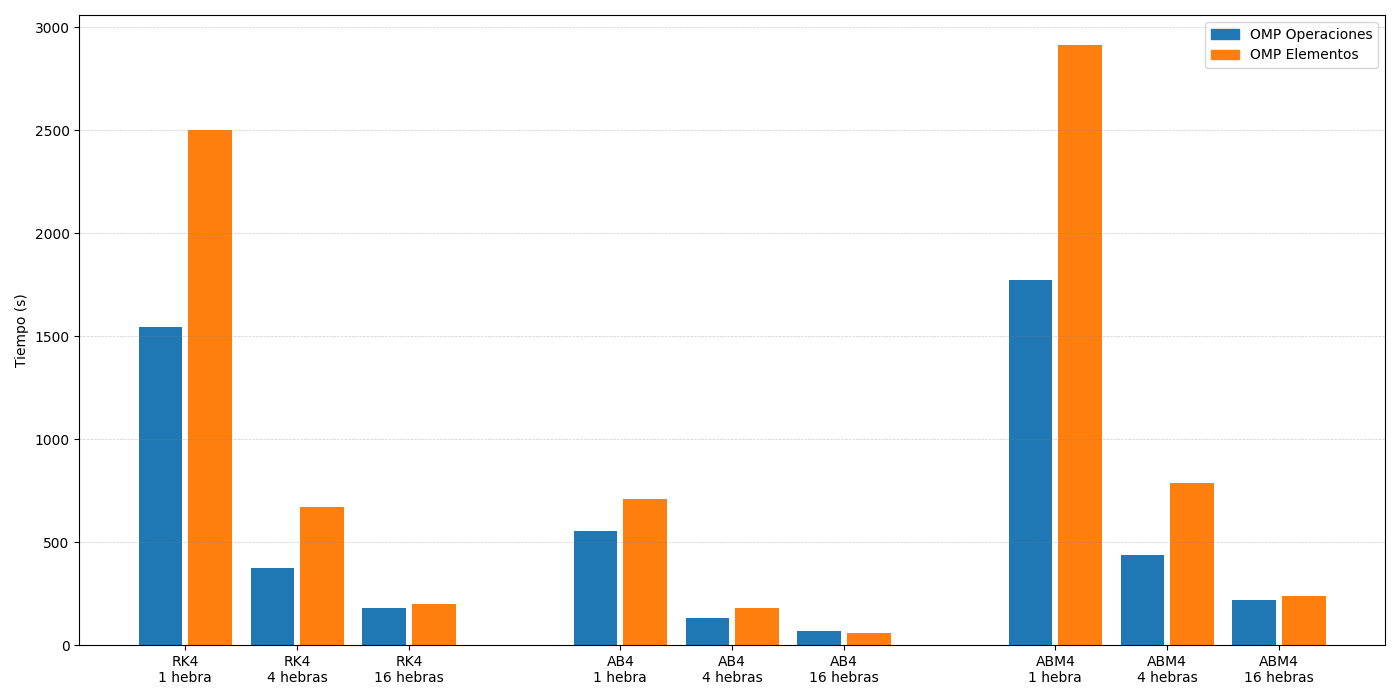
\includegraphics[width=\linewidth]{imagenes/Brusselator1D-100K.png}
	\caption{Brusselator1D 100.000 ecuaciones}
	\label{fig:Brusselator1D-100K}
\end{figure}

Como podemos ver, hay una mejora sustancial del tiempo al pasar de 1 a 4 y a 16 hebras, con ambas estrategias de paralelismo, y con los 3 métodos numéricos. Además, se aprecia que la resolución con Adams-Bashford es más rápida que Runge-Kutta, ya que es más directa y no requiere de los pasos intermedios (K1, K2, K3, K4), y también es mucho más veloz que el predictor-corrector Adams-Bashford-Moulton, ya que éste último llama a Adams-Bashford dentro de su bucle de ejecución. Además, podemos ver que para este tipo y tamaño de problema, el paralelismo por operaciones es más eficiente para 4 hebras, pero ambos se equiparan cuando se alcanzan las 16.

Podemos probar por ejemplo, con el problema más complejo (\textit{Brusselator2D}), y el método que más tarda (\textit{ABM4}), y podemos comparar la evolución del tiempo conforme aumenta el tamaño del problema, a saber, con un número de ecuaciones igual a 45000, 80000 y 125000.

\begin{table}[H]
	\begin{center}
		\begin{tabular}{| c | c | c | c | c | c |}
			\hline
			\textbf{neqn} & \textbf{Hebras} & \textbf{Estrategia} & \textbf{T (s)} & \textbf{Speedup} & \textbf{Eficiencia} \\
			\hline
			
			% ---------------- 45000 ----------------
			\multirow{6}{*}{45000}
			& \multirow{2}{*}{1}  & Operaciones & 976.061 & \multirow{2}{*}{1} & \multirow{2}{*}{100} \\
			\cline{3-4}
			&                     & Componentes & 2151.79 &                   &                    \\
			\cline{2-6}
			& \multirow{2}{*}{4}  & Operaciones & 263.081 & 3.710115896 & 92.7528974 \\
			\cline{3-6}
			&                     & Componentes & 569.693 & 3.777104511 & 94.4276128 \\
			\cline{2-6}
			& \multirow{2}{*}{16} & Operaciones & 180.662 & 5.402691213 & 33.7668201 \\
			\cline{3-6}
			&                     & Componentes & 206.744 & 10.40799249 & 65.0499531 \\
			\hline
			
			% ---------------- 80000 ----------------
			\multirow{6}{*}{80000}
			& \multirow{2}{*}{1}  & Operaciones & 1825.86 & \multirow{2}{*}{1} & \multirow{2}{*}{100} \\
			\cline{3-4}
			&                     & Componentes & 3970.37 &                   &                    \\
			\cline{2-6}
			& \multirow{2}{*}{4}  & Operaciones & 466.282 & 3.915784868 & 97.8946217 \\
			\cline{3-6}
			&                     & Componentes & 1049.35 & 3.78364702 & 94.5911755 \\
			\cline{2-6}
			& \multirow{2}{*}{16} & Operaciones & 214.67 & 8.505426934 & 53.1589183 \\
			\cline{3-6}
			&                     & Componentes & 331.809 & 11.96582974 & 74.7864359 \\
			\hline
			
			% ---------------- 125000 ----------------
			\multirow{6}{*}{125000}
			& \multirow{2}{*}{1}  & Operaciones & 2692.79 & \multirow{2}{*}{1} & \multirow{2}{*}{100} \\
			\cline{3-4}
			&                     & Componentes & 5982.94 &                   &                    \\
			\cline{2-6}
			& \multirow{2}{*}{4}  & Operaciones & 675.123 & 3.988591708 & 99.7147927 \\
			\cline{3-6}
			&                     & Componentes & 1593.61 & 3.754331361 & 93.8582840 \\
			\cline{2-6}
			& \multirow{2}{*}{16} & Operaciones & 264.402 & 10.18445398 & 63.6528373 \\
			\cline{3-6}
			&                     & Componentes & 445.081 & 13.44236218 & 84.0147636 \\
			\hline
			
		\end{tabular}
		\caption{Brusselator2D con ABM4}
		\label{tab:Brusselator2D-ABM4}
	\end{center}
\end{table}

Para calcular el speedup y la eficiencia, hemos comparado los valores de mismo tamaño y estrategia, para que la comparación sea más justa. Más allá de lo obvio, que conforme aumenta el tamaño del problema, aumentan los tiempos, es cuanto menos destacable la variación en los speedups que se alcanzan en función del aumento de las hebras, en una estrategia y otra.

\begin{figure}[H]
	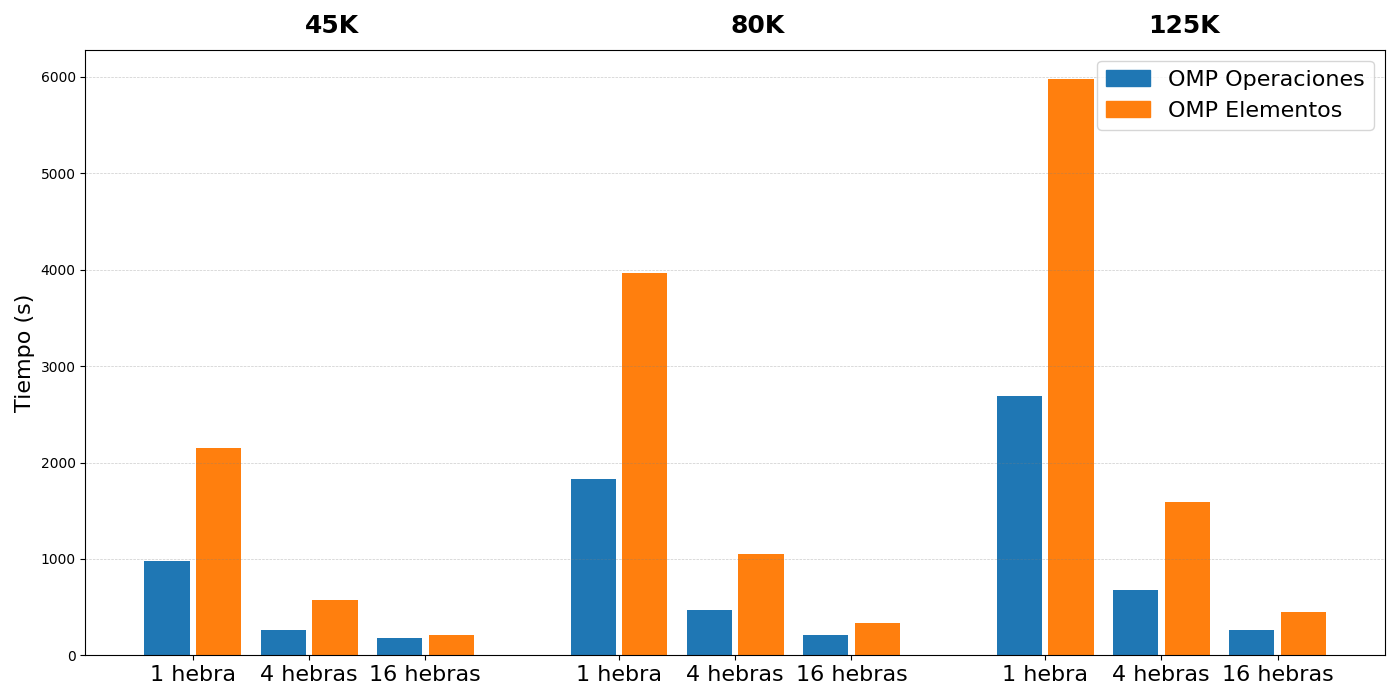
\includegraphics[width=\linewidth]{imagenes/Brusselator2D-ABM.png}
	\caption{ABM4 resolviendo Brusselator2D}
	\label{fig:Brusselator2D-ABM4}
\end{figure}

Partiendo de los mismos datos, pero tomando ahora solo el speedup y la eficiencia, y quedándonos con paralelismo de operaciones, tendríamos estas métricas:

\begin{figure}[H]
	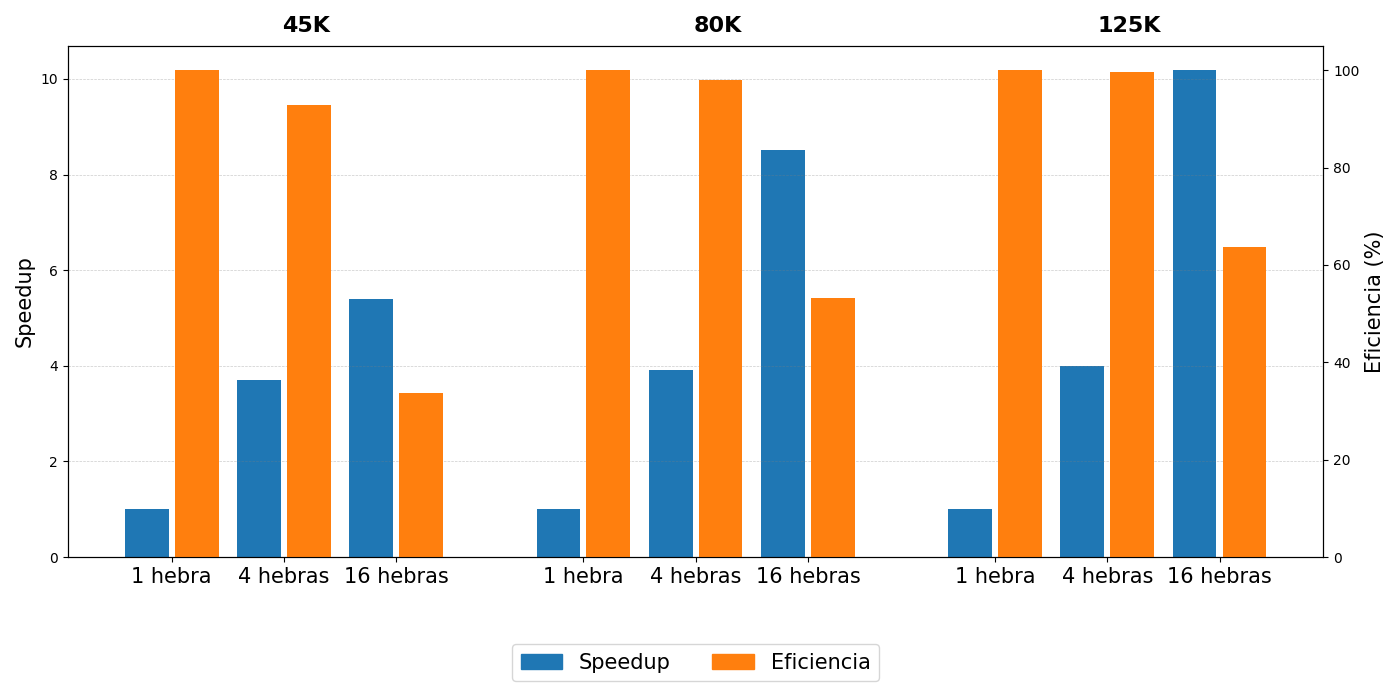
\includegraphics[width=\linewidth]{imagenes/OMP-Speedup-Eficiencia.png}
	\caption{Speedup y Eficiencia - ABM4 Brusselator2D}
	\label{fig:Spd-Eff-ABM4-Br2D}
\end{figure}

Tenemos la barras del speedup en azul y alineadas con el eje Y izquierdo, y en naranja y con el eje Y derecho la eficiencia en valores porcentuales. Obviamente, para 1 hebra siempre tendremos un speedup de 1, y una eficiencia de 100\%.

Más allá de eso, podemos ver varias ideas en juego a la vez. Si nos centramos en cualquiera de los 3 tamaños, podemos ver la Ley de Amdahl \cite{Amdahl1967} en funcionamiento; con un mismo tamaño de problema, conforme crece el número de hilos, aumenta el speedup pero disminuye la eficiencia, ya que siempre queda una parte secuencial que no se puede paralelizar.

Análogo a esto, si nos fijamos ahora en las columnas de la eficiencia, podemos ver que, para un mismo número de hebras, conforme aumenta el tamaño de problema, la eficiencia lo hace con él, pasando de un 33\%, a un 53\%, y a un 63\%, cuando observamos los datos relativos a las 16 hebras por ejemplo. Esto coincide con la ley de Gustafson \cite{Gustafson1988}, ya que al aumentar el tamaño del problema, crece la parte del programa que es paralelizable, y por lo tanto la eficiencia aumenta también.